\documentclass[reqno]{amsart}
\usepackage{amscd, amssymb, amsmath, amsthm}
\usepackage{graphicx}
\usepackage[colorlinks=true,linkcolor=blue]{hyperref}
\usepackage[utf8]{inputenc}
\usepackage[T1]{fontenc}
\usepackage{textcomp}
\usepackage{babel}
%% for identity function 1:
\usepackage{bbm}
%%For category theory diagrams:
\usepackage{tikz-cd}

%\usepackage[backend=biber]{biblatex}
%\addbibresource{.bib}


\setlength\parindent{0pt}

\pdfsuppresswarningpagegroup=1

\newtheorem{theorem}{Theorem}[section]
\newtheorem{lemma}[theorem]{Lemma}
\newtheorem{proposition}[theorem]{Proposition}
\newtheorem{corollary}[theorem]{Corollary}
\newtheorem{conjecture}[theorem]{Conjecture}

\theoremstyle{definition}
\newtheorem{definition}[theorem]{Definition}
\newtheorem{example}[theorem]{Example}
\newtheorem{exercise}[theorem]{Exercise}
\newtheorem{problem}[theorem]{Problem}
\newtheorem{question}[theorem]{Question}

\theoremstyle{remark}
\newtheorem*{remark}{Remark}
\newtheorem*{note}{Note}
\newtheorem*{solution}{Solution}



%Inequalities
\newcommand{\cycsum}{\sum_{\mathrm{cyc}}}
\newcommand{\symsum}{\sum_{\mathrm{sym}}}
\newcommand{\cycprod}{\prod_{\mathrm{cyc}}}
\newcommand{\symprod}{\prod_{\mathrm{sym}}}

%Linear Algebra

\DeclareMathOperator{\Span}{span}
\DeclareMathOperator{\im}{im}
\DeclareMathOperator{\diag}{diag}
\DeclareMathOperator{\Ker}{Ker}
\DeclareMathOperator{\ob}{ob}
\DeclareMathOperator{\Hom}{Hom}
\DeclareMathOperator{\Mor}{Mor}
\DeclareMathOperator{\sk}{sk}
\DeclareMathOperator{\Vect}{Vect}
\DeclareMathOperator{\Set}{Set}
\DeclareMathOperator{\Group}{Group}
\DeclareMathOperator{\Ring}{Ring}
\DeclareMathOperator{\Ab}{Ab}
\DeclareMathOperator{\Top}{Top}
\DeclareMathOperator{\hTop}{hTop}
\DeclareMathOperator{\Htpy}{Htpy}
\DeclareMathOperator{\Cat}{Cat}
\DeclareMathOperator{\CAT}{CAT}
\DeclareMathOperator{\Cone}{Cone}
\DeclareMathOperator{\dom}{dom}
\DeclareMathOperator{\cod}{cod}
\DeclareMathOperator{\Aut}{Aut}
\DeclareMathOperator{\Mat}{Mat}
\DeclareMathOperator{\Fin}{Fin}
\DeclareMathOperator{\rel}{rel}
\DeclareMathOperator{\Int}{Int}
\DeclareMathOperator{\sgn}{sgn}
\DeclareMathOperator{\Homeo}{Homeo}
\DeclareMathOperator{\SHomeo}{SHomeo}
\DeclareMathOperator{\PSL}{PSL}
\DeclareMathOperator{\Bil}{Bil}
\DeclareMathOperator{\Sym}{Sym}
\DeclareMathOperator{\Skew}{Skew}
\DeclareMathOperator{\Alt}{Alt}
\DeclareMathOperator{\Quad}{Quad}
\DeclareMathOperator{\Sin}{Sin}
\DeclareMathOperator{\Supp}{Supp}
\DeclareMathOperator{\Char}{char}
\DeclareMathOperator{\Teich}{Teich}
\DeclareMathOperator{\GL}{GL}
\DeclareMathOperator{\tr}{tr}
\DeclareMathOperator{\codim}{codim}
\DeclareMathOperator{\coker}{coker}
\DeclareMathOperator{\corank}{corank}
\DeclareMathOperator{\rank}{rank}
\DeclareMathOperator{\Diff}{Diff}
\DeclareMathOperator{\Bun}{Bun}
\DeclareMathOperator{\Sm}{Sm}
\DeclareMathOperator{\Fr}{Fr}
\DeclareMathOperator{\Cob}{Cob}
\DeclareMathOperator{\Ext}{Ext}
\DeclareMathOperator{\Tor}{Tor}
\DeclareMathOperator{\Conf}{Conf}
\DeclareMathOperator{\UConf}{UConf}



%Row operations
\newcommand{\elem}[1]{% elementary operations
\xrightarrow{\substack{#1}}%
}

\newcommand{\lelem}[1]{% elementary operations (left alignment)
\xrightarrow{\begin{subarray}{l}#1\end{subarray}}%
}

%SS
\DeclareMathOperator{\supp}{supp}
\DeclareMathOperator{\Var}{Var}

%NT
\DeclareMathOperator{\ord}{ord}

%Alg
\DeclareMathOperator{\Rad}{Rad}
\DeclareMathOperator{\Jac}{Jac}

%Misc
\newcommand{\SL}{{\mathrm{SL}}}
\newcommand{\mobgp}{{\mathrm{PSL}_2(\mathbb{C})}}
\newcommand{\id}{{\mathrm{id}}}
\newcommand{\MCG}{{\mathrm{MCG}}}
\newcommand{\PMCG}{{\mathrm{PMCG}}}
\newcommand{\SMCG}{{\mathrm{SMCG}}}
\newcommand{\ud}{{\mathrm{d}}}
\newcommand{\Vol}{{\mathrm{Vol}}}
\newcommand{\Area}{{\mathrm{Area}}}
\newcommand{\diam}{{\mathrm{diam}}}
\newcommand{\End}{{\mathrm{End}}}


\newcommand{\reg}{{\mathtt{reg}}}
\newcommand{\geo}{{\mathtt{geo}}}

\newcommand{\tori}{{\mathcal{T}}}
\newcommand{\cpn}{{\mathtt{c}}}
\newcommand{\pat}{{\mathtt{p}}}

\let\Cap\undefined
\newcommand{\Cap}{{\mathcal{C}}ap}
\newcommand{\Push}{{\mathcal{P}}ush}
\newcommand{\Forget}{{\mathcal{F}}orget}




\begin{document}
    

\begin{definition}[Coexact]
    A sequence
    \[
    A \stackrel{f}{\to} B \stackrel{g}{\to} C
    \] 
    of pointed spaces (or pointed pairs) is called
    \textit{coexact} if, for each pointed space
    (or pair) $Y$, the sequence of sets 
    (pointed homotopy classes)
    \[
    \left[ C;Y \right] 
    \stackrel{g^{\#}}{\to} 
    \left[ B;Y \right] 
    \stackrel{f^{\#}}{\to} 
    \left[ A;Y \right] 
    \] 
    is exact.
\end{definition}

\begin{theorem}[]
    For any map $f \colon A \to X$ and for the
    inclusion $i \colon X \hookrightarrow C_f$, the
    sequence
    \[
    A \stackrel{f}{\to} X \stackrel{i}{\to} C_f
    \] 
    is coexact.
\end{theorem}

\begin{proof}
    Clearly, $i \circ f \simeq *$, the constant map
    to the base point (by sliding $A$ up
    along its cone to the vertex).
    Now suppose $\varphi 
    \in \ker f^{\#} \in 
    \left[ X;Y \right] $. By assumption then
    $\varphi \circ f$ is nullhomotopic,
    say via a homotopy $F$.
    Then putting $F$ on $A \times I$ and
    $\varphi $ on $X$, we get a map
    $C_f \to Y$ extending $\varphi $ - its
    image under $i^{\#}$ is given by restricting
    to $X \subset C_f$, which is $\varphi $.
\end{proof}

\begin{corollary}
    If $f \colon A \hookrightarrow X$ is a cofibration, where
    $A \subset X$ is closed, then
     \[
         A \to X \to X / A
     \] 
     is coexact.
\end{corollary}

\begin{corollary}
    Let $f \colon A \to X$ be any map. Then the sequence
    \[
    A \stackrel{f}{\to} X \stackrel{i}{\to} C_f
    \stackrel{j}{\to} C_i \stackrel{k}{\to} C_j
    \] 
    is coexact, where
    $j$ and $k$ are the obvious inclusions.
\end{corollary}

We can replace $C_i$ and $C_j$ by simpler things.
Note that $C_i = C_f \cup_X CX$, see Figure
\ref{fig:Figures-Cf-cone-png}.

\begin{figure}[htpb]
    \centering
    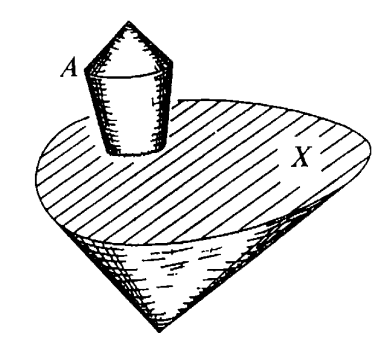
\includegraphics[width=0.3\textwidth]{Figures/Cf-cone.png}
    \caption{}
    \label{fig:Figures-Cf-cone-png}
\end{figure}

In this figure, we can construct a deformation
carrying $CX$ to the base point through itself.
Throughout this deformation, we can stretch the
mapping cylinder of $f$ to accommodate it.

Now using Theorem \ref{Thm:Bredon-4.5}, we obtain
that the collapsing map
$C_i \to C_i / CX = C_f / X = SA$ is a homotopy equivalence.
Similarly, $C_j \simeq CX$. Under these
homotopy equivalences, we will show that
$k$ becomes $Sf$. Consider
Figure \ref{fig:Figures-DJIOWJA-png}.

\begin{figure}[htpb]
    \centering
    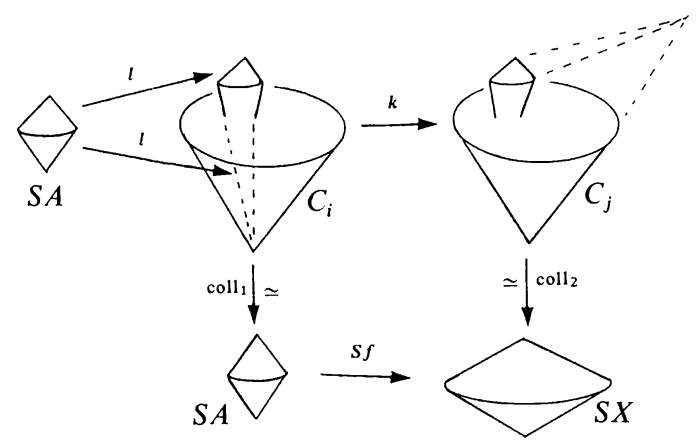
\includegraphics[width=0.8\textwidth]{Figures/DJIOWJA.png}
    \caption{}
    \label{fig:Figures-DJIOWJA-png}
\end{figure}

The map $l$ in the figure stretches the top
cone of $SA$ to the cylinder part of
$C_f \subset C_i$ and
is $Cf$ on the bottom cone.

The map  $coll_1$ is the collapse of the
bottom of the picture and gives the homotopy equivalence
$C_i \simeq SA$ obtained above.
The map $coll_2$ is the collapse of the top of $C_j$ in
the picture (the dashed lines) and is the
homotopy equivalence $C_j \simeq SX$.

Firstly, we clearly have $coll_1 \circ l \simeq \id$, so
$l$ is a homotopy inverse of $coll_1$, i.e.,
 $l \circ coll_1 \simeq \id$ as well.

 Also, $coll_2 \circ k \circ l = Sf \circ g \simeq
 Sf$, where $g$ is the collapse
 of the top cone of $SA$.

 Composing with $coll_1$ on the right gives
 $coll_2 \circ k \simeq 
 coll_2 \circ k \circ l \circ coll_1
 \simeq S_f \circ coll_1$, so the diagram
 
 \begin{equation*}
 \begin{tikzcd}
     C_i \ar[r, "k"] \ar[d, "coll_1"] & C_j \ar[d, "coll_2"] \\
     SA \ar[r, "Sf"] & SX
 \end{tikzcd}
 \end{equation*}
 is homotopy commutative.

 Thus,
 \begin{corollary}
     Give any map
     $f \colon A \to X$ of pointed spaces,
     the sequence
     \[
     A \stackrel{f}{\to} X \stackrel{i}{\to} 
     C_f \stackrel{g}{\to} SA \stackrel{Sf}{\to} 
     SX
     \] 
     is coexact, where
     $g \colon C_f \to SA$ is the composition
     of the collapse $C_f \to C_f /X$ with
     the homotopy equivalence
     $SA \simeq C_f / X$ induced by the inclusion
     of $A \times I$ in $\left( A \times I \right) 
     \sqcup X$ followed by the quotient map to
     $C_f$ and then the collapsing of the subspace
      $X$ of $C_f$.
 \end{corollary}

 \begin{lemma}[]
     Coexactness is preserved by suspension.
 \end{lemma}

 \begin{proof}
     Suppose $A \to B \to C$ is coexact.
     Then the sequence
     \[
     \left[ SC;Y \right] \to 
     \left[ SB;Y \right] 
     \to \left[ SA;Y \right] 
     \] 
     is equivalent to the sequence
     \[
     \left[ C;\Omega Y \right] 
     \to \left[ B ; \Omega Y \right] 
     \to \left[ A; \Omega Y \right] 
     \] 
     which is exact by assumption.
 \end{proof}

 \begin{corollary}[Barratt-Puppe]
     If $f \colon A \to X$ is any map then the sequence
     \[
     A \stackrel{f}{\to} B \stackrel{i}{\to} 
     C_f \stackrel{g}{\to} SA
     \stackrel{Sf}{\to} SX \stackrel{Si}{\to} 
     SC_f \stackrel{Sg}{\to} 
     S^2 A \stackrel{S^2 f}{\to} 
     \] 
     is coexact. Furthermore, 
     $SC_f \cong C_{Sf}$, etc. Similarly for maps
     of pairs of pointed spaces.
 \end{corollary}






    %\printbibliography
\end{document}
